\documentclass[12pt]{report}
\usepackage{graphicx}
\usepackage{enumitem}
\usepackage{amsmath}
\begin{document}

\title{Guide to Bioinformatics tools and resources}
\author{Matthew Welland}
\date{\today}
\maketitle	
	
\chapter*{File Types}


\section*{BAM}
\begin{itemize}
	\item A Binary version of a SAM file, storing the same data in a more concise format
	\item BAM is used in most production pipelines, but SAM may be used where interconversion with other applications is crucial
\end{itemize}

Both of the file types contain the same actual data, but the overall space the data takes up and the format differs between the two. 

Sam files contain an optional header section:
\begin{itemize}
	\item HD - Header
	\item SQ - Seqence Dictionary
	\item RG - Read Group
	\item PG - Program
	\item CO - Comment
\end{itemize}
This is followed by an alignment section; multiple tab-delimited lines with each line describing an alignment.

\begin{figure}[!ht]
	\centering
	\fbox{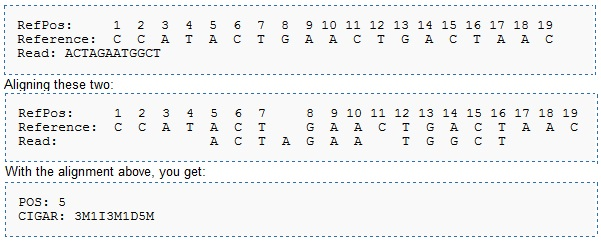
\includegraphics[scale=0.8]{CIGAR}}
	\caption{The CIGAR will indicate a start position (where the lengths and operations begin to correspond to the reference sequence) and a sequence of relations}\label{cigar}
\end{figure}
\section*{CIGAR}
CIGAR strings are used to show how well a read is paired to the appropriate reference sequence. This is a String composed of base lengths and the operation describing how the lengths indicate similarities or differences between the sequences. The operations are used to show:

\begin{itemize}
	\item mismatches/matches
	\item lengths of bases relating to the operation
	\item deletions from the read
	\item insertions in the read
\end{itemize}

\section*{CRAM}
CRAM is a potential successor to BAM - a compressed version of the allignment.
\begin{enumerate}
	\item CRAM starts with a file definition followed by the BAM header and other containers
	\item Each subsequent container starts with a container header followed by 1 or more block
	\item Each block starts with a block header; all real data comes after this header
	\item The first block in each container is the compression header block
	\item Each subsequent block is organised into slices. A slice may contain a contiguous region of alignment data. Each slice has a slice header block followed by 1 or more data blocks
	\item Each data block is divided into a mandatory core data block and optional external data blocks
\end{enumerate}

\section*{FastA}
A text-based format for representing either nucleotide or protein sequences, using a single-character encoding for each atomic component. This is a super simple format, making it simple to parse with any scripting language.

The first line of each FastA entry begins with a `\textgreater' character, followed by the description line. There shouldn't be a space between the `\textgreater' and the start of the identifier. The sequence ends if another line beginning with `\textgreater' appears, indicating the start of another sequence. Lines are typically limited to 80 characters in length. Several single-sequence Fasta files can be concatenated to display a multiple sequence file, with each new entry starting with a`\textgreater' and a description line.

\section*{FastQ}
A text based format for storing a biological sequence and its corresponding quality scores. This format typically use four lines per sequence:
\begin{enumerate}
	\item Begins with a '@' character and is followed by a sequence identifier and an optional description (similar to a title line)
	\item Raw sequence letters
	\item Begins with a + character and is \textbf{optionally} followed by the sequence identifier
	\item Encodes the quality values for the sequence in line 2, and must contain the same number of characters as there are letters in the sequence
\end{enumerate}
The character `!' in the quality String indicates the lowest quality, whilst `\textasciitilde' indicates the highest. 
\begin{figure}[!ht]
	\centering
	\fbox{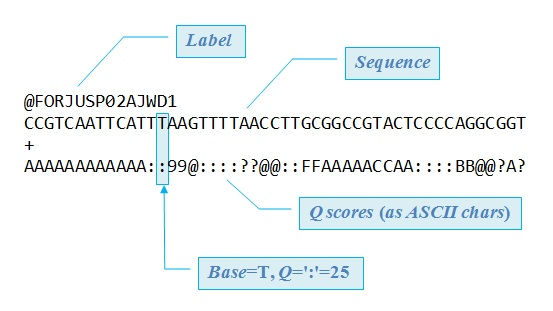
\includegraphics[scale=0.6]{FastQ}}
	\caption{An annotated FastQ file example, showing the raw sequence and the corresponding quality values}\label{FastQ}
\end{figure}

\section*{SAM}
\begin{itemize}
	\item SAM stands for Sequence Alignment Map
	\item A text file format for storing sequence data in a series of tab-delimited ASCII files
	\item SAM files are generally created by aligners which read a FastQ file and assign sequences to a position within a reference genome
\end{itemize}

\begin{figure}[ht]
	\centering
	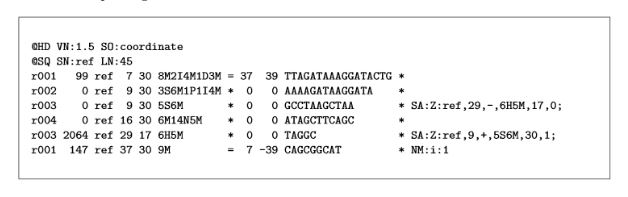
\includegraphics{SAM}
	\caption{An example of a SAM format file, showing the tab-delimited columns containing data}\label{SAM}
\end{figure}

\section*{PHRED}
PHRED is a quality score, originally developed during the Human Genome Project. Phred quality scores $\displaystyle Q$ are defined as a property which is logarithmically related to the base-calling error probabilities $\displaystyle P$:

\begin{figure}[h]
	\begin{equation}
		Q = -10 log_{10} P
	\end{equation}
\end{figure} 

This means that a Phred score of 3 indicates that the probability of the base having been called incorrectly is 1 in 1000. The most common method of using Phred is to disregard any bases which do not have a quality score of at least 20.

\begin{figure}[ht]
	\centering
	\fbox{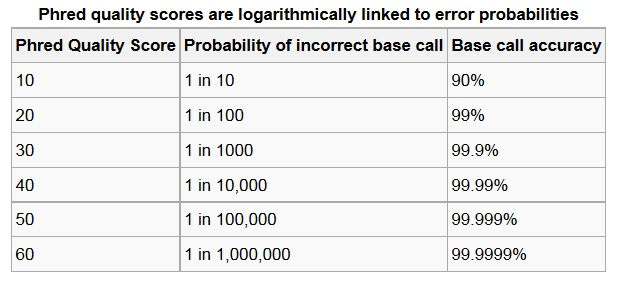
\includegraphics[scale=0.5]{Phred}}
	\caption{A table describing the relationship between Phred score and accuracy}\label{Phred}
\end{figure}

\section*{BED}

The Browser Extensible Data (BED) file format consists of one line per feature, each containing 3-12 columns of data. The first three fields are mandatory;
\begin{enumerate}
	\item chrom: name of the chromosome or scaffold. Chromosome names can be provided with or without the 'chr' prefix
	\item chromStart: start position of the feature in standard chromosomal coordinates
	\item chromEnd: end position of the feature in standard chromosomal coordinates
\end{enumerate}
There are nine additional fields which can be used to supply further information:
\begin{enumerate}[resume]
	\item name: label to be displayed under the feature
	\item score: a score between 0 and 1000
	\item strand: '+' for forward, '-' for reverse
	\item thickStart: field used by UCSC drawing code (not needed in Ensembl)
	\item thickEnd: as thickEnd (?)
	\item itemRgb: an RGB colour value for display
	\item blockCount
	\item blockSizes
	\item blockStarts
\end{enumerate}
Track definition lines can be used to configure the display further, e.g. by grouping features into separate tracks. The 'Track line' begins with the word ``track'', followed by a range of space-separated key-value pairs.

BED file start positions are zero-based, whilst end positions are one-based. This means that to identify the length of a specified segment, the values only have to be subtracted directly. This is different to some other formats (such as GFF or VCF), but the change in numbering is accounted for in all tools which manipulate this file type.

\section*{Variant Call Format}

The Variant Call Format (VCF) specifies the format of a text file used in bioinformatics for storing gene sequence variations. This standardised format allows for improved interoperability between NGS tools, in the same way that the SAM/BAM specification revolutionised alignment tools. The VCF file format is text based, making it easy to generate and parse, and includes extensible meta-data passages alongside the mandatory header information. 

\begin{figure}[ht]
	\centering
	\fbox{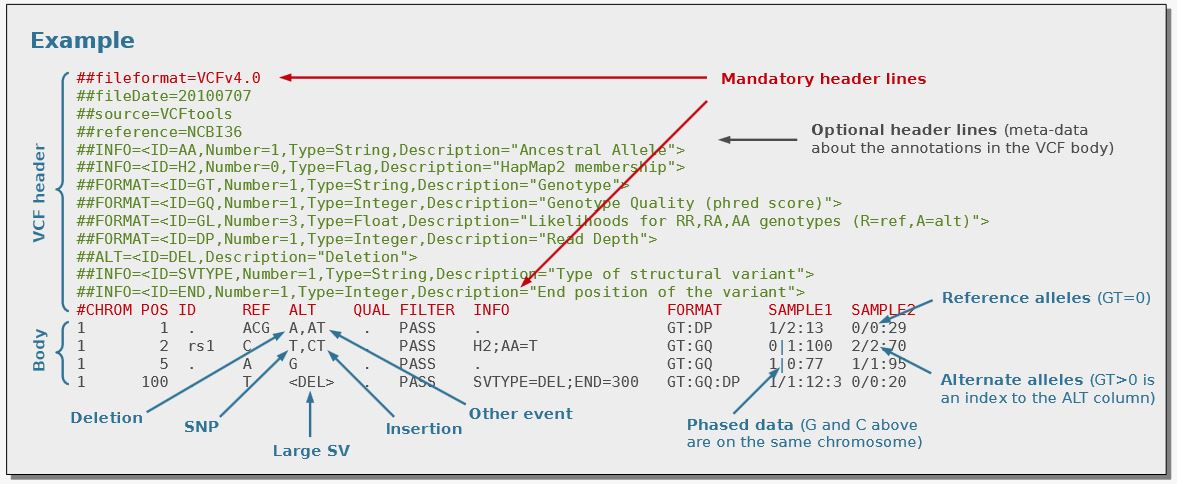
\includegraphics[scale=0.4]{VCF_demo}}
	\caption{A demonstration of the VCF file format, labelling different structural features}\label{VCF}
\end{figure}

\chapter*{Tools}

\section*{FastQC}

FastQC is a tool created by the Babraham institute which allows a quick analysis of the quality of sequence data encoded in input files. As huge amount of sequence data can be produced during a sequencing run, the overall quality of the data should be examined before conclusions are drawn. Most sequencers will generate a QC report as part of their analysis pipeline, but this is usually only focused on identifying problems which were generated by the sequencer itself. FastQC aims to provide a QC report which can spot problems which originate either in the sequencer or in the starting library material. This application allows users to:
\begin{itemize}
	\item Import of data from BAM, SAM or FastQ files (any variant)
	\item Providing a quick overview to tell you in which areas there may be problems
	\item Summary graphs and tables to quickly assess your data
	\item Export of results to an HTML based permanent report
	\item Offline operation to allow automated generation of reports without running the interactive application	
\end{itemize}


\section*{SAMTools}
A set of utilities for interacting with and post-processing short DNA sequence read alignments in SAM, BAM, and CRAM formats, typically generated by short read aligners such as BWA. This toolkit provides utilities such as sorting and indexing, as well as more complex variant calling and alignment. SAMtools allows a user to work directly with the SAM file format without having to decompress the contents. 

A range of the SAMtools commands are listed on both the Wikipedia page and readme. The SAMtools tools are used via a command line, and UNIX style piping and stream processing are possible using standard syntax.

\section*{BEDTools}
BEDtools is a toolset for genomic arithmetic; set theory on the genome. This enables users to intersect, merge, count, complement and shuffle genomic intervals from multiple files in formats such as BAM, BED \& VCF. Combining multiple BEDtools operations can allow production of complex results. There are a wide range of tools included in the BEDtools package with such varied functions as changing file type, finding overlapping windows within a genomic interval, and creating an HTML page of links to UCSC locations.

The genome features which can be recognised, manipulated and interrogated using BEDtools can be genes, polymorphisms, SNPs, INDELs or structural variants. A laboratory may also incorporate novel findings into the data set as custom annotations. The basic attributes of genome features are:
\begin{itemize}
	\item the scaffold or reference on which the feature is found
	\item the base pair where the feature starts
	\item the base pair on which the feature ends
	\item the strand (forward '+' or reverse '-')
	\item the name of the feature (where appropriate)
\end{itemize}

BEDtools also allows command line piping of commands, simplifying the process of creating a large chain of operations. 

\section*{BEDOPS}
An open-source command-line toolkit that performs efficient and scalable Boolean and set operations, statistical calculations, archiving, conversion, and other genomic management.

http://bedops.readthedocs.org/en/latest/content/overview.html

BEDops also includes a novel lossless format called 'Starch' which is capable of reducing file sizes of whole-genome BED files to $\approx$5\% of original, and BAM files to around $\approx$35\% of original, whilst adding useful metadata and random access. 

\section*{IGV}
\begin{figure}[ht]
	\centering
	\fbox{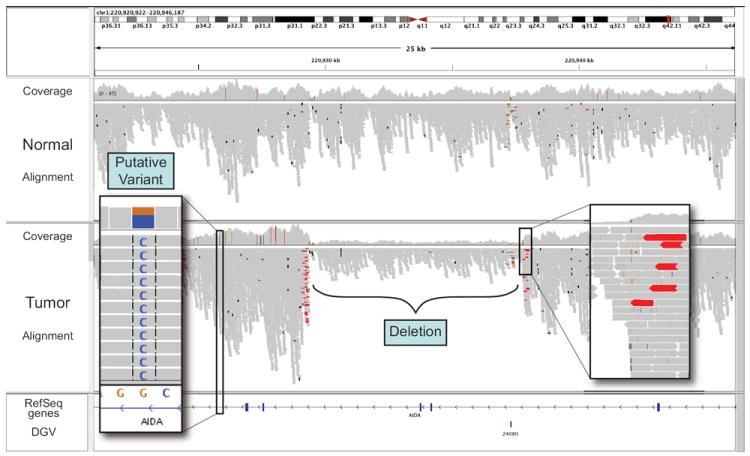
\includegraphics[scale=0.5]{IGV}}
	\caption{An image of IGV showing a sequence alignment at 20Kb resolution}\label{IGV}
\end{figure}

The Integrative Genomics Viewer (IGV) is a response to the increasing presence of genome-wide data available by modern molecular genetic methods. This is a light-weight visualisation tool created at the Broad Institute which enable real-time exploration of diverse, large-scale genomic data sets including:

\begin{itemize}
	\item Aligned Sequence Reads
	\item Mutations
	\item Copy number variations
	\item RNA interference screens
	\item Gene Expression
	\item Methylation
	\item Genomic annotations
\end{itemize}
This tool permits simultaneous visualisation of arbitrarily large data sets over all resolution scales, using efficient multi-resolution file formats. Whilst there are multiple genome browsers currently available, IGV focuses on the emerging integrative nature of genomic studies, placing equal emphasis on array and NGS platforms, and including clinical attributes and metadata.

\section*{Annovar}


\section*{Variant Effect Predictor}

The Variant Effect Predictor (VEP) is a suite of tools used to determine the likely impact of variants found within biological sequences (SNPs, insertions, deletions, CNVs or structural variants). By inputting the coordinates of variants and the nucleotide changes, this suite can be used to find:

\begin{itemize}
	\item genes and transcripts affected by the variants
	
	\item location of the variants (e.g. upstream of a transcript, in coding sequence, in non-coding RNA, in regulatory regions)
	
	\item consequence of your variants on the protein sequence (e.g. stop gained, missense, stop lost, frameshift)
	
	\item known variants that match yours, and associated minor allele frequencies from the 1000 Genomes Project
	
	\item SIFT and PolyPhen scores for changes to protein sequence
\end{itemize}

All of the options available in the VEP suite can be selected using a graphical interface or a set of command line options. The VEP tool set can be downloaded, and a cache of local variant and reference sequence data can be stored to cut down on the network traffic created during variant identification. NOTE: The cache files required to run VEP locally are a few GB in size, download may take a long time (and if done via CMD may seem to hang for up to half an hour). Available identifiers include:

\begin{itemize}
	 \item Gene symbol - add the gene symbol for the gene to the output. This will typically be, for example, the HGNC identifier for genes in human.
	 
	 \item CCDS - add the Consensus CDS transcript identifier where available.
	 
	 \item Protein - add the Ensembl protein identifer (ENSP).
	 
	 \item Uniprot - add identifiers for translated protein products from three UniProt-related databases (SWISSPROT, TREMBL and UniParc).
	 
	 \item HGVS - generate HGVS identifiers for your input variants relative to the transcript coding sequence (HGVSc) and the protein sequence (HGVSp).
	 
	 \item Find co-located known variants - report known variants from the Ensembl Variation database that overlap with your input.
	 
	\item The VEP can also report minor allele frequency (MAF) data for existing variants from two major genotyping projects, the 1000 Genomes Project and the NHLBI-ESP
	
\end{itemize}

The VEP makes use of a range of data formats, and can additionally use other formats such as VCF directly as input. The default input format is whitespace-separated (space or tab characters):

\begin{itemize}
	\item Chromosome - just the name or number, with no 'chr' prefix
	\item Start coordinate
	\item End coordinate
	\item Allele - pair of alleles separated by a '/', with the reference allele first
	\item Strand - defined as + (forward) or - (reverse).
	\item Identifier (optional) - this identifier will be used in output. If not provided, the VEP will construct an identifier from coordinates and alleles.
	
\end{itemize}

\begin{figure}[ht]
	\centering
	\fbox{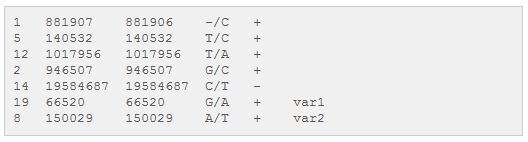
\includegraphics[scale=0.8]{VEP_input}}
	\caption{An example of valid input lines for the VEP}\label{VEP_in}
\end{figure}

Flags can be used to request specific output types using the VEP; JSON, VCF, or tab-delimited text output. VEP can also publish results in an HTML page format, incorporating descriptive charts and other details which may be of use.

\section*{VEP CMD Example}

This section shows a few standard uses of the VEP on the command line, using common options.

\begin{itemize}
	\item perl variant\_effect\_predictor.pl -i example\_GRCh38.vcf --cache
\end{itemize} 

This will run the VEP on the default example file, containing 1000 Genomes Project variants. The default output path is variant\_effect\_output.txt, if this file already exists, the --force\_overwrite option can be used. the --quiet option reduces the progress output, only printing warnings and errors.

\begin{itemize}
	\item head variant\_effect\_output.txt
\end{itemize}

This is just a quick head read command to view the output created through the previous set of processes. This will show the metadata lines included at the top of the file, indicated by ``\#\#''

\begin{itemize}
	\item perl variant\_effect\_predictor.pl -i example\_GRCh38.vcf --cache --force\_overwrite --sift b
\end{itemize}

This sequence includes the --sift b command, which tells the VEP to conduct a SIFT analysis on the variants included in the VCF. 


\begin{itemize}
	\item perl filter\_vep.pl -i variant\_effect\_output.txt -filter "SIFT is deleterious" | head -n15
\end{itemize}

Use of VEP's filtering script can narrow down this set of results to only show those in which the output as determined by SIFT as deleterious.

\begin{itemize}
	\item perl variant\_effect\_predictor.pl -i example\_GRCh38.vcf --cache --force\_overwrite --sift b --canonical --symbol \
	--fields Uploaded\_variation,SYMBOL,CANONICAL,SIFT -o STDOUT | \
	perl filter\_vep.pl -format vep -filter "CANONICAL is YES and SIFT is deleterious"
\end{itemize}

This (huge) command is an example input which executes a standard VEP process with SIFT calculations, selects specific fields from that process to display, and then passes the output through a specific VEP filtering script to extract only the entries which satisfy the specific conditions listed. In this example, this shows only variants which have a deleterious effect on canonical gene transcripts, and shows the symbols for the appropriate genes.

These examples were taken from the Ensembl docs on VEP.

\section*{Bioconductor}

\section*{GATK}

\chapter*{Aligners and Algorithms}
\section*{Burrows-Wheeler Aligner}

\section*{Human Reference Genome Versions}

\chapter*{Databases}

\section*{Types of database}
Each entry a separate section?

\section*{Flat file}

A flat file database is a very token addition to this list; simply put it is a document containing data, or a location where unconnected documents can be stored. It will not usually contain any form of intelligent search, version control or other features common among specifically designed database implementations.

\section*{Object Database}

An object database is a database management system in which information is represented in the form of objects (similar to the concept of object oriented programming (OOP)). By combining database and OOP-language capabilities a system can use a continuous model for data representation in the storage medium and the programming language used to control it. An example would be creating a Java object, setting its attribute values, and saving the object as an entry within the database. A join query would not be required to fully recreate the object, as a pointer could be used to identify the location of the complete set of values instead.

Class methods which are associated with the object within the programming language can be used to interact with objects and attributes. Some Object Database Management Systems (ODMSs) allow for version control of the objects, and can show good performance when the objects stored are huge (compared with a field-by-field relational reconstruction of an entity).

\section*{Relational Database}

A relational database is a data storage facility which makes use of Edgar Codd's relational model. This sorts data into one or more tables with a unique key labelling each row. The terminology within the relational model refers to each table as a relation, the fields or columns as attributes, and each row as a tuple.

\begin{itemize}
	\item Each entity type to be modelled within the database is typically modelled by a table (relation), and each rown (tuple) represents an instance.
	
	\item Complex entities and relationships can be represented by joining entities represented by several tables - unique row identifiers can be used to select specific instances.
	
	\item Each attribute in each table will have a specific domain; a range of values which it may take. An attribute may be specified as an integer, a Boolean value, or a String for instance.
	
	\item Constraints may also be added to the field domain, such as ensuring certain fields are not left blank, or providing a range of values an attribute must fall between. 
	
	\item Foreign keys are the method of linking between tuples in different tables, and indexes may be used to speed up queries executed on different tables. Indexes are often implemented as trees for their flexibility. 
	
	\item Relational operations such a Joins, Intersections, Differences and Full joins can be used to create sets of records gathering all the details of an entity or a concept. 
	
	\item Normalization is a logical process which can be applied to relational database tables. This involves a progressive decomposition of a table into several single tables to ensure that no conflicting relationships exist between the attributes, and to make sure that insertions or deletions to any given field will not cause errors elsewhere in the database.
\end{itemize}


\section*{Graph Database}

This type of database implements graph structures with nodes, edges, and properties to represent and store data.

\begin{itemize}
	\item Every element contains a direct pointer to its adjacent elements and no index lookups are necessary. 
	
	\item Each entity is represented by a node (Person, place, concept...), and each node has a range of descriptive properties (age, value, location...).
	
	\item Edges connect nodes, and represent the relationship between objects. This relationship can have a descriptive name and attributes. Most of the relational information in the database is stored in/on the edges.
	
	\item Each node has an arbitrary number of edges. Compared with Object or Relational databases they may be capable of modelling real world situations more faithfully, and perform better for associative data sets.
	
	\item Operations such as computing the shortest path between objects via existing relationships is simple using the Graph schema.
\end{itemize}

\section*{NoSQL}

Not only SQL (NoSQL) refers to a range of non-relational database methodologies. An example is a document based database (such as PLONE), where individual documents are uploaded and can be tagged with specific identifiers to enable searching across a range of items to select those relating to the chosen properties.

\section*{Normalization}
For relational databases, normalisation is a process of reducing redundancy within a database and ensuring that data integrity is implicitly maintained during updates and additions. An example of this is the repetition of a single field value when referring to multiple rows. e.g.:
\vspace*{1\baselineskip}

\begin{tabular}{|c|c|c|c|}\hline
	\centering
RecordID  & UserID  &   Name  &    Role   \\ \hline
1     &     1   &   Matt  & DB Analysis\\ \hline
2     &     1   &   Matt  & Coffee making\\ \hline
3     &     2   &   Hagrid& Yodelling \\ \hline
\end{tabular}
\vspace*{1\baselineskip}

In this database example, the UserID and the Name both refer to the same person, and the data is repeated across multiple rows. This means that there is a possibility of updating one of the 'Matt' records and altering the Name field, or inserting a new record with the wrong name/ID combination, corrupting the data the table represents. To ensure that this is not a risk, the single table can be split into two tables, one containing UserID : Name relationships, and the other containing UserID : Role relationships. 

Although this is a simple example, the same logic applies when examining larger tables. If a single record consists of groups of data which each depend on the primary key, but are not linked together, separation of the single record into distinct tables can improve security against update and expansion problems.


\chapter*{Other}

\section*{Reciever Operator Characteristic}
\end{document}